\documentclass[12pt,a4paper]{report}
\usepackage[utf8]{inputenc}
\usepackage[english]{babel}
\usepackage{hyperref}
\usepackage{xcolor}
\usepackage{listings}
\usepackage{minted}
\usepackage[urldate=comp,dateabbrev=false, backend=biber]{biblatex}
\usepackage{array}
\usepackage{longtable}
\usepackage{graphicx}
\usepackage{caption}
\usepackage{subcaption}

\definecolor{lightyellow}{RGB}{255,242,204}

\newminted{bash}{frame=single}
\newminted{properties}{frame=single}
\newminted{xml}{frame=single}

\addbibresource{document.bib}

\DefineBibliographyStrings{english}{
urlseen = {Retrieved},
}

\begin{document}

\tableofcontents

\chapter{Installation}
\label{ch:installation}
In this chapter, we show steps necessary to install and run a sample web utility, which allows to retrieve images based on their content. To meet this purpose we will use content-based image retrieval library called \textbf{LIRE} (\textbf{L}ucene \textbf{I}mage \textbf{RE}trieval). This library provides methods for indexing and searching images. The LIRE uses for these purposes full text search engine library called \textbf{Apache Lucene}. Since we want to create the web application, we use for image retrieving search web-based platform \textbf{Apache Solr}, based on the Apache Lucene.

\section{Apache Solr Setup}
Apache Solr is an open source enterprise search platform. It is written in Java and runs as a standalone full-tex search server within a servlet container such as Jetty. Solr has REST-like HTTP/XML and JSON API to obtain and index data.\cite{solr}

\subsection{Installation}
At first we need to download the Solr from its web page\footnote{\url{http://lucene.apache.org/solr/mirrors-solr-latest-redir.html}}. Solr requires for running Java version 1.6 or greater.

\begin{listing}[H]
\caption{Checking the Java version.}
\begin{bashcode}
java -version
\end{bashcode}
\end{listing}

We begin by unzipping the Solr release. Created directory we will mark as \textit{\$SOLR\_HOME}. Solr distribution contains example server as a template for our own installation. So we must copy \textit{example} directory and this copy we call \textit{server} \footnote{It is important to call directory as \textit{server}, because default startup script supposes such name.}. All steps we demonstrate in the listing \ref{lst:solrInstallation}.

\begin{listing}[H]
\caption{Solr Installation}
\label{lst:solrInstallation}
\begin{bashcode}
unzip solr-X.X.X.zip
cd $SOLR_HOME
# copying example directory
cp -r example server
\end{bashcode}
\end{listing}

Now when Solr is successfully installed, we have to create and configure a new solr core. The solr cores are located in the directory called \textbf{solr}. In this directory it already exists a pre created default core with the name \textbf{collection1}. We can simply rename this core. After the renaming, we need to specify its properties in the \textbf{core.properties} file, where we set name to \textit{liresolr}.

\begin{listing}[H]
\caption{Creating a new solr core.}
\begin{bashcode}
cd $SOLR_HOME/server/solr
mv collection1 liresolr
vim liresolr/core.properties
\end{bashcode}
\end{listing}

Now we can run the jetty server and we can see a solr admin page on the \textit{\url{http://localhost:8983/solr/}}.

\begin{listing}[H]
\caption{Running the Solr server.}
\begin{bashcode}
$SOLR_HOME/bin/solr start
\end{bashcode}
\end{listing}

\section{Lire Setup}

The LIRE (Lucene Image REtrieval) library provides a simple way to retrieve images and  photos based on their color and texture characteristics. LIRE creates a Lucene index of image features for content based image retrieval (CBIR).\cite{lire}

\subsection{Compilation}

At first, we need to download and compile LIRE handlers. We can do it in two simple steps. We have to clone git repository to our local computer and then we use ant build script to build the project. After it we should see in the \textbf{dist} directory the \textbf{lire-request-handler.jar} file.

\begin{listing}[H]
\caption{Download and compile LIRE Solr project.}
\begin{bashcode}
# clone repository
git clone https://github.com/moravianlibrary/liresolr
cd liresolr
# build project and create a jar file
ant dist
\end{bashcode}
\end{listing}

\subsection{Integration to the Solr}

After we compile LIRE project, we have to integrate jar package in the Solr class-path. At first we have to copy \textbf{lire-request-handler.jar} to the Solr project and then we need to configure class-path for these files (see listings \ref{lst:copyLireRequestHandler} and \ref{lst:setClassPath}). We can specify it in the \textbf{solrconfig.xml}\footnote{You can find it in \textit{/path/to/project/solr/solr/liresolr/conf} directory}.

\begin{listing}[H]
\caption{Copying needed files.}
\label{lst:copyLireRequestHandler}
\begin{bashcode}
# change working directory to solr
cd /path/to/project/solr
mkdir handlers
# change working directory to liresolr
cd /path/to/project/liresolr
# copy lire-request-handler.jar and libraries to the solr
cp -r dist/lire-request-handler.jar lib ../solr/handlers
\end{bashcode}
\end{listing}

\begin{listing}[H]
\caption{Setting up the class-path.}
\label{lst:setClassPath}
\begin{xmlcode}
<config>
  <lib dir="../../handlers" regex=".*\.jar" />
  <lib dir="../../handlers/lib" regex=".*\.jar" />
</config>
\end{xmlcode}
\end{listing}

Now when we have LIRE handlers in the class-path we register them in the \textbf{solrconfig.xml} file.

\begin{listing}[H]
\caption{Handlers registration.}
\begin{xmlcode}
<config>
  <requestHandler name="/lireId"
  class="net.semanticmetadata.lire.solr.handler.
  IdentityRequestHandler">
     <lst name="defaults">
       <str name="echoParams">explicit</str>
       <str name="wt">json</str>
       <str name="indent">true</str>
     </lst>
  </requestHandler>
  <requestHandler name="/lireSim"
  class="net.semanticmetadata.lire.solr.handler.
  SimilarRequestHandler">
     <lst name="defaults">
       <str name="echoParams">explicit</str>
       <str name="wt">json</str>
       <str name="indent">true</str>
     </lst>
  </requestHandler>
</config>
\end{xmlcode}
\end{listing}

In this tutorial we use only two handlers, which we will use to request identical or similar image. If you want to know more about using LIRE Solr integration you can see\cite{liresolr}.

We also need to define fields in the \textbf{schema.xml}, in which the Solr will store the data about images. For storing data about images we will use two types of information. First will have suffix \textbf{\_ha} and it will represents a hash of image, which the Solr need for fast searching. This information will be a text type. Second type of information will be a binary type and it will be used to store some data, which will represents the image. These fields will have suffix \textbf{\_hi}. To retrieve images we will combine two different methods -- Color layout and SURF (Speeded Up Robust Features) image descriptor. Because of these facts we have to specify four fields to store data about images. In this specification we define our own field so we cannot forget to add the definition of the custom field at the same field (see listings \ref{lst:schemaSpec} and \ref{lst:binaryDVDef}).

\begin{listing}[H]
\caption{Fields specification.}
\label{lst:schemaSpec}
\begin{xmlcode}
<fields>
   <!-- file path for ID -->
   <field name="id" type="string" indexed="true"
   stored="true" required="true" multiValued="false" />
   <!-- Needed for SOLR -->
   <field name="text" type="text_general" indexed="true"
   stored="false" multiValued="true"/>
   <!-- ColorLayout -->
   <field name="cl_ha" type="text_ws" indexed="true"
   stored="false" required="false"/>
   <field name="cl_hi" type="binaryDV"  indexed="false"
   stored="true" required="false"/>
   <!-- SURF -->
   <field name="su_ha" type="text_ws" indexed="true"
   stored="false" required="false"/>
   <field name="su_hi" type="binary"  indexed="false"
   stored="true" required="false" multiValued="true"/>
   <!-- Needed for SOLR -->
   <field name="_version_" type="long" indexed="true"
   stored="true"/>
</fields>
\end{xmlcode}
\end{listing}

\begin{listing}[H]
\caption{Definition of our field binaryDV.}
\label{lst:binaryDVDef}
\begin{xmlcode}
<types>
 <fieldtype name="binaryDV"
 class="net.semanticmetadata.lire.solr.BinaryDocValuesField"/>
</types>
\end{xmlcode}
\end{listing}

On the end we will have to add configuration file \textbf{liresolr.properties} to the config directory of your solr core\footnote{Into the same directory where it is the solrconfig.xml}. We will speak more about configuration in the next chapters.

\begin{listing}[H]
\caption{liresolr.properties}
\begin{propertiescode}
# It defines how many images will be obtained from solr
# and then they will be compared
# with the queried image.
# Visual Words
numVisualWordsImages = 30
# Color Layout
numColorLayoutImages = 2000
# It defines how many images will be obtained from solr
# at similar searching (/lireSim)
numColorLayoutSimImages = 10
numSurfSimImages = 30
# Count of images returned by /lireSim handler:
numSimilarImages = 30
# It defines if system should resize queried image.
# Parameter defines shorter side of the image.
# You can use value 0 for no resize.
resizeQueryImage = 400
# It defines treshold of Color Layout method. Images,
# which have the distance less than the
# threshold, will be marked as potentional identical
# images to the queried image.
thresholdCLIdentity1 = 7.0
# It defines the second level of threshold. If it exists
# exactly one image, which has
# distance less than first threshold and it has also
# distance less than the second
# threshold, system says, that this image is identical
# to the queried image.
thresholdCLIdentity2 = 5.0
# It defines threshold of the SURF method. Images which
# have distance greater or equals
# to this value will be removed from a list of candidates
# to the identical image.
thresholdSUIdentity = 0.9
\end{propertiescode}
\end{listing}

\section{Indexing Images}

We can index images using by various methods. More information about indexing image data you can find here\cite{createIndex}. If we would want to create our own application for indexing images, it is very important to use the same jar file \textbf{lire.jar}, which is used by solr handlers, because this library contains data, which are used to generate hash functions. For our purposes we can use a simple indexer, which extracts data from images using by Color Layout and SURF method. It also provides method to import this data to the Solr server. We can easily download it from the git repository \url{https://github.com/moravianlibrary/liresolrindexer}. (See listing \ref{lst:liresolrindexer})

\begin{listing}[H]
\caption{Download and compile Lire Solr Indexer.}
\label{lst:liresolrindexer}
\begin{bashcode}
# clone repository
git clone https://github.com/moravianlibrary/liresolrindexer
cd liresolrindexer
# create jar package
ant package
\end{bashcode}
\end{listing}

Now we will need a directory, which will contain images. We can create it in our project folder and we can call it \textbf{data}. Then we move all images for indexing to this folder. We also copy our \textbf{indexer.jar} from \textit{liresolrindexer/dist} directory. We cannot forget copy the \textbf{lib} folder due to dependencies. In the same directory has to be a \textbf{config.propeties} file (see listing \ref{lst:configFile}), which contains indexer configuration. We check and properly set these properties before indexing process. All neccesary information about configuration are in this file.

\begin{listing}[H]
\caption{config.properties}
\label{lst:configFile}
\begin{propertiescode}
# Url to the solr core, where indexer will import data.
solrCoreUrl = http://localhost:8983/solr/liresolr
# Path to the solr core data folder,
# where indexer copy clusters-surf.dat.
solrCoreData = /path/to/project/solr/solr/liresolr/data
# Number of the documents, which will be used to create
# vocabulary (clusters-surf.dat).
numDocsForVocabulary = 800
# This is equivalent to a number of the visual words,
# which will be used to search images.
numClusters = 1000
# Number of threads, which will be used to index images.
numberOfThreads = 2
\end{propertiescode}
\end{listing}

Since indexer accepts like parameter a file, which contains list of images for indexing, we have to create simple text file, in which will be represent each line one path to the image. We can do it by many ways. See listing \ref{lst:creatingImagesList}.

\begin{listing}[H]
\caption{Creating list of the images.}
\label{lst:creatingImagesList}
\begin{bashcode}
find . -name "*.jpg" > images
\end{bashcode}
\end{listing}

Finally we can type following command.

\begin{listing}[H]
\caption{Indexing images.}
\begin{bashcode}
java -jar indexer.jar index images
\end{bashcode}
\end{listing}

After the indexing process we have to import the generated data to the Solr server. Indexer reads information about the server from \textbf{config.properties} file so we should properly set these properties. Then we can simple use the command from the listing \ref{lst:importData}. For more information about this tool see\cite{indexer}.

\begin{listing}[H]
\caption{Importing data to the Solr.}
\label{lst:importData}
\begin{bashcode}
java -jar indexer.jar import
\end{bashcode}
\end{listing}

\section{Simple Web Application}

The last step will be adding a simple web application to the Jetty server. This application will allow a user to insert the requested image and then it will display information obtained from the server. Our \textbf{LireSolr} project already contains this simple web app so we will show how to create a war package, which we deploy to the Jetty and how to properly set some other properties.

Firstly, we need to create war package. We just change our working directory to the \textit{/path/to/project/liresolr} and then we run the ant script. If compilation process was successful, we can find \textbf{web.war} file in the \textbf{dist} directory.

\begin{listing}[H]
\caption{Creating war package.}
\begin{bashcode}
ant web
\end{bashcode}
\end{listing}

Secondly, we have to integrate the war package into the Jetty server. We just simply copy the file into the \textbf{webapp} folder and then we add a context description for this file. We can do it like this.

\begin{listing}[H]
\caption{Integrating war package to the Jetty server.}
\begin{bashcode}
cd /path/to/project/solr
cp ../liresolr/dist/web.war webapps
cd contexts
vim web-context.xml
\end{bashcode}
\end{listing}

\begin{listing}[H]
\caption{web-context.xml}
\begin{xmlcode}
<?xml version="1.0"?>
<!DOCTYPE Configure PUBLIC "-//Jetty//Configure//EN"
"http://www.eclipse.org/jetty/configure.dtd">
<Configure class="org.eclipse.jetty.webapp.WebAppContext">
  <Set name="contextPath">/lire</Set>
  <Set name="war">
    <SystemProperty name="jetty.home"/>/webapps/web.war
  </Set>
</Configure>
\end{xmlcode}
\end{listing}

Thirdly, the web page expects that it can access to the image data on the context path \textbf{/lire/data}. So we have to allow the access on this url. We can do it by adding the next xml descriptor to the \textbf{contexts} directory. We can call it for example \textbf{data-context.xml}. See listing \ref{lst:data-context}. After these steps we should be able to connect to the \url{localhost:8983/lire}. Now we can try to find some image.

\begin{listing}[H]
\caption{data-context.xml}
\label{lst:data-context}
\begin{xmlcode}
<?xml version="1.0"  encoding="ISO-8859-1"?>
<!DOCTYPE Configure PUBLIC
"-//Mort Bay Consulting//DTD Configure//EN"
"http://jetty.eclipse.org/configure.dtd">
<Configure
class="org.eclipse.jetty.server.handler.ContextHandler">
 <Set name="contextPath">/lire/data</Set>
 <Set name="resourceBase">/path/to/project/data</Set>
 <Set name="handler">
  <New
  class="org.eclipse.jetty.server.handler.ResourceHandler">
   <Set name="directoriesListed">false</Set>
   <Set name="cacheControl">max-age=3600,public</Set>
  </New>
 </Set>
</Configure>
\end{xmlcode}
\end{listing}

\chapter{Development}
"The main goal of content-based image retrieval is to find similar images. While similarity itself is a
concept that is hard to formalize, the problem is compounded by the need for comparing millions
of images to a query image at search time -- a very challenging task. A common approach consists
in representing images using the minimal amount of information needed to encode its essential
properties.This minimal information -- called image descriptor -- is usually extracted from the image’s
raw pixel values (and their coordinates) -- a process known as feature extraction -- and encoded in a
numeric vector, the feature vector. Similarity, then, is defined by a suitable metric that computes a
distance between two vectors. The design, extraction, and encoding of the image features as well as
the choice of the metric makes up for a mathematical representation of visual similarity"\cite[s. 30]{VIRbook}.

In this chapter we introduce some technique how to extract the minimal information from the image -- called image descriptor. Then we will compare these methods and we will show how to combine it together to use the best from the each method. During the all research we will focus on the map comparing. We will search techniques how to efficiently find identical or similar maps.

\section{Image Descriptor}

"Ideally, descriptors should be:
\begin{itemize}
\item \textbf{representative} of the contents of the image (or region) from which they were extracted,
\item \textbf{robust} to image rotation, scaling, or translation (often referred to as RST invariant in the computer vision literature),
\item \textbf{compact}, since the number of dimensions and the range of possible values along each dimension are critical to search time behavior"\cite[s.~30]{VIRbook}.
\end{itemize}

Now we have to realize how we will retrieve the image data. In the chapter \ref{ch:installation} we said that we use for the image retrieving the Apache Solr server, which is the search platform, which includes powerful full-text search. Therefore, our goal will be creating the descriptor, which we could transform into the textual information. Although, we are able to find similar images based on the text information, we also want to compute a distance value from the queried image. This information will said how the images are similar to this image. To compute such information we will need to store data, from which we could compute later this value. Below we will be called the textual information as a \textbf{hash} and the information, which will be represented the image, we will be called a \textbf{histogram}.

\section{Color Layout}

This method uses to extract the image descriptor a color information from the picture. Big advantage of this fact is that we can very fast compute such information. Descriptor is represented by the color histogram. It is the most intuitive visual descriptor. We can imagine it like an array of real values. The question is, how this information can be transformed into the textual form. The biggest problem is that the real numbers can have infinite number of values\footnote{We know that the computer cannot actually store all real numbers, but for simplicity we suppose that it can.} and we represent the textual information with just small subset of the natural numbers. So we have to map the bigger set of values to the smaller set. For this purpose we can use the hash function. Advantage of this method is that it is very fast. By this way we can compute the hash information mentioned in the introduction of this section.

To create a histogram we can use the color histogram, which we used to compute the hash. This we can use this information later to compute the distance between images. You can read here\cite{ColorLayout} more about computing of the distance.

\section{SURF}

"SURF is a performance-oriented scale and rotation-invariant interest point detector and descriptor.
Its performance with respect to repeatability, distinctiveness, and robustness"\cite[s.~42]{VIRbook}.

SURF uses to create the image descriptor a local feature. It is usually associated with a change of one or more image properties, such as intensity, color, and texture. Local features can be interest points, corners, edges, or salient spots. If we want to integrate this technique we have to transform these local features into the textual information, which will represents the image. We can do it in the following steps.

\begin{enumerate}
\item We choose some sample images and we extract from them the local features. We can image these features like points in some vector space. Sometimes it is called as interest points.
\item We distribute this points into clusters. We use for this purpose a method called \textbf{k-means clustering}\footnote{\url{http://en.wikipedia.org/wiki/K-means_clustering}}.
\item We assign to the each cluster a string. For example the first cluster will be \textit{v0}, the second cluster will be \textit{v1} and so on.
\item We take a sequence of the local features from the image and then we assign to them strings, based on the clusters, into the which they belong. So we get a sequence of words, which we can called \textbf{visual words}.
\end{enumerate}

Based on the visual words, we can get from the Solr server set of images, which are similar to the queried image. Although by this way we get good results, the searched image may not always appear on the first place. Because of improvement of results, we have to compare each image point by point\footnote{We mean interest points}. We have two set of points and we have to find pairs of similar points. We define similar points so that if distance between two points is less than some constant, the points are similar. By this method we have to perform (n x m) operations. Computation of distance by this way is very slow. We try to do some optimization, but in the future this problem should be solved with the more sophisticated algorithm. The main idea of this optimization is to sort the interest points and so speed up searching a similar points. Optimized process of comparing performs in following steps.

\begin{enumerate}
\item We compute for each point a distance from a vector (1,1,1...1). We cannot compute it from a vector (0,0,0...0) because the interest points are normalized.
\item We sort these points based on this computed distance.
\item We take one point from the first image and we find some neighborhood of points, which have similar distance from the vector (1,1,1...1), in the second image. We use binary search algorithm to find this neighborhood.
\item We compare the point from the first image with the founded points from the second image.
\end{enumerate}

\section{Tests}
\label{sec:tests}

In this section we will test mentioned method to create image descriptor. We will talk about their advantages and disadvantages and on the end we will summarize our observations.

\subsection{Color Layout}

During testing we tried to find similar images by each method separately. It has been shown that the Color Layout is very fast, it can return a result in less than one second, and it is reliable to find an identical image. It returned a correct result in the each test. Results of the tests are shown in the table \ref{tab:colorLayoutTest}. Although differences between first and second image are big enough, there are some cases, when these differences are small. In these situations we cannot surely say that it exists an identical image and that it is the first image.

\begin{center}
\begin{longtable}{|m{7cm}|r|r|}

\caption{Results of the Color Layout test.} \label{tab:colorLayoutTest}\\

\hline
& \multicolumn{2}{c|}{Distance} \\
\hline
URL & First image & Second image \\
\hline
\endfirsthead
\hline
& \multicolumn{2}{c|}{Distance} \\
\hline
URL & First image & Second image \\
\hline
\endhead
\endfoot
\endlastfoot
\url{http://mapy.mzk.cz/tmp/duplicity-test/orig/2619267582.jpg} & 3.1462643 & 7.6242585\\
\hline
\url{http://mapy.mzk.cz/tmp/duplicity-test/orig/2619267505a.jpg} & 1.4142135 & 9.518843\\
\hline
\url{http://mapy.mzk.cz/tmp/duplicity-test/orig/2619267580.jpg} & 1.0 & 6.358899\\
\hline
\url{http://mapy.mzk.cz/tmp/duplicity-test/orig/2619267578a.jpg} & 3.4142137 & 7.0318995\\
\hline
\url{http://mapy.mzk.cz/tmp/duplicity-test/orig/2619267576.jpg} & 2.4142137 & 7.1046295\\
\hline
\url{http://mapy.mzk.cz/tmp/duplicity-test/orig/2619267574.jpg} & 3.1462643 & 7.63103\\
\hline
\url{http://mapy.mzk.cz/tmp/duplicity-test/orig/2619267572.jpg} & 2.0 & 8.056606\\
\hline
\url{http://mapy.mzk.cz/tmp/duplicity-test/orig/2619267570.jpg} & 3.3166249 & 7.322473\\
\hline
\url{http://mapy.mzk.cz/tmp/duplicity-test/orig/2619267567.jpg} & 3.3166249 & 8.071068\\
\hline
\url{http://mapy.mzk.cz/tmp/duplicity-test/orig/2619267565.jpg} & 5.595754 & 6.768857\\
\hline
\url{http://mapy.mzk.cz/tmp/duplicity-test/orig/2619267564.jpg} & 4.5604777 & 7.0\\
\hline
\url{http://mapy.mzk.cz/tmp/duplicity-test/orig/2619267555.jpg} & 2.0 & 6.210045\\
\hline
\url{http://mapy.mzk.cz/tmp/duplicity-test/orig/2619267658.jpg} & 3.732051 & 5.878315\\
\hline
\url{http://mapy.mzk.cz/tmp/duplicity-test/orig/2619267604.jpg} & 1.4142135 & 8.658535\\
\hline
\url{http://mapy.mzk.cz/tmp/duplicity-test/orig/2619267603a.jpg} & 3.732051 & 6.7993784\\
\hline
\url{http://mapy.mzk.cz/tmp/duplicity-test/orig/2619267600.jpg} & 5.1462646 & 6.656854\\
\hline
\end{longtable}
\end{center}

Disadvantage of this method is that it searches images based on the color and then it cannot find the same image, which is scanned on another scanner. Differences between such two images are illustrated in the figure \ref{fig:identicalMaps}. In this case, the Color Layout cannot find the indexed map.

\begin{figure}[H]
  \centering
  \begin{subfigure}{0.5\textwidth}
    \centering
    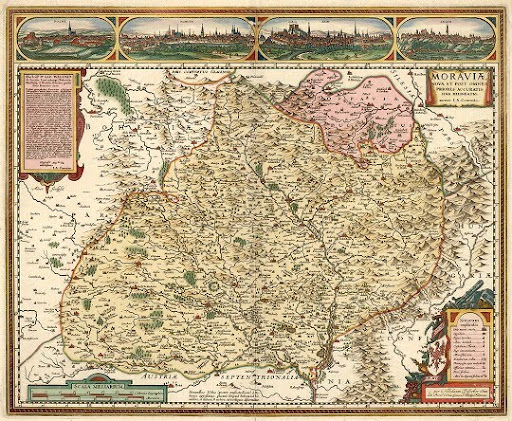
\includegraphics[width=0.8\linewidth]{indexed_map.jpg}
    \caption{Indexed map.}
    \label{fig:indexedMap}
  \end{subfigure}%
  \begin{subfigure}{0.5\textwidth}
    \centering
    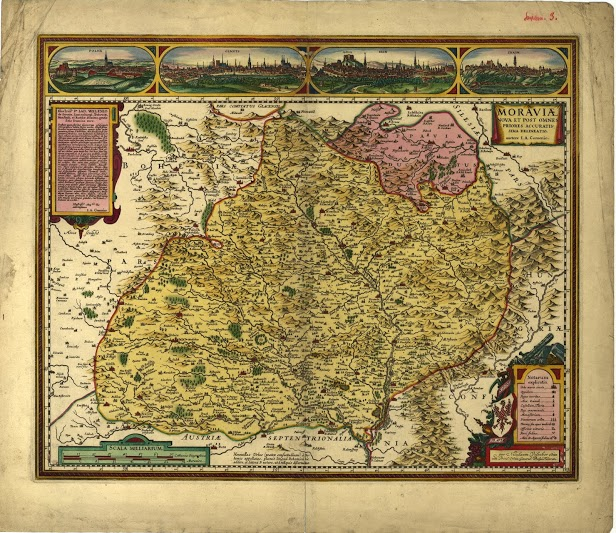
\includegraphics[width=0.8\linewidth]{searched_map.jpg}
    \caption{Searched map.}
    \label{fig:searchedMap}
  \end{subfigure}
\caption{Two "identical" maps.}
\label{fig:identicalMaps}
\end{figure}

\subsection{SURF}

When we tried SURF method on the set of the images from the previous section, results was surprising. SURF cannot find almost any image. Problem was that the indexed images are thumbnails with the small resolution and the searched images had bigger resolution. In these images were found more interest points than in the indexed and it caused that was generated different sequences of visual words. When we scaled the searched image into the same resolution like had the indexed images, we got much better results. System was able even recognize similarity between images in the figure \ref{fig:identicalMaps}.

Main disadvantage is that the whole search process took several times more time compared to Color Layout method. For example, while the Color Layout searched an image less than one second, the SURF searched this image more than nine seconds.

\subsection{Summary}

The choice of the image descriptor depends on our expectations from a system. If we want to find identical image, which is just scaled, we can use the Color Layout descriptor, which is very fast. On the other hand if we want to find some similarity between images and we are willing to wait a few seconds, SURF method is better choice. But we have to realize, that we do not have to use only one technique but we can combine it so that we use the best from the each method.

\chapter{Implementation}

In this chapter we will show how we implemented handlers, which search identical or similar images based on the image information. We will explain step by step how the whole process works. During the explanation we will also say something about constants, which we can set in the configuration files (see chapter \ref{ch:installation}).

\section{Identity}

The process of searching identical image combines together both methods -- Color Layout and SURF. It should be as fast as possible, but on the other hand it should be able to surely say, if some image exists in the system or not. For this purpose we have to define some thresholds, which will be determined, which image is identical and which is not. We use the data from the section \ref{sec:tests}.

Procedure, how the handler evaluates if the identical image is in the system or not:

\begin{enumerate}
\item Based on the color hash, the Solr finds 2000 images\footnote{This value is stored in the lire.properties file under key \textit{numColorLayoutImages}}.
\item Based on the color histogram, all founded images are compared with the searched image and it choose images, which have the distance less than 7.0\footnote{\textit{thresholdCLIdentity1}}.
\item If there is no such a image, result is that it does not exist identical image.
\item If there is exactly one image and distance is less than 5.0\footnote{\textit{thresholdCLIdentity2}}, result is, that it exists identical image and that it is this one.
\item If there is exactly one image and distance is greater or equal than 5.0, it computes distance between images by the SURF method. If the distance is less than 0.9\footnote{\textit{thresholdSUIdentity}}, image is considered as identical. Otherwise, the system says, that there is no identical image.
\item If there is more than one image, it computes the distance for all images by the SURF method. Images, which have distance greater or equal to 0.9, will be removed from list of candidates to the identical image. If the list will be empty after this step, result will be that there is no identical image. Otherwise, it computes the new distance as \textit{Color Layout distance} x \textit{SURF distance} and the image with the smallest distance will be returned as the identical image.
\end{enumerate}

\section{Similarity}

Similar like in the identity handler, we will use both methods to get similar images from the Solr. Process, which searches these images, is more straightforward. Firstly we find by the color hash 10 images\footnote{\textit{numColorLayoutSimImages}} and 30 images\footnote{\textit{numSurfSimImages}} by the SURF hash. Secondly we compute distances by the SURF histograms (comparing interest points) and on the end we sort these images based on the computed distance.

\printbibliography

\end{document}
